\documentclass[twoside, twocolumn, 12pt]{article}

\usepackage{blindtext}
%\usepackage[backend=bibtex,style=verbose-trad2]{biblatex}
\usepackage{fontspec}
%\defaultfontfeatures{Mapping=tex-text,Scale=MatchLowercase}
\usepackage{amsmath}

\usepackage{geometry}
 \geometry{
 a4paper,
 total={170mm,257mm},
 left=20mm,
 top=20mm,
 }
 
 
%\usepackage[czech]{babel}
%\addto\extrasczech{\def\bibname{tttttttttttt}\let\refname\bibname}


\usepackage{graphicx}

\usepackage{polyglossia}
\XeTeXlinebreaklocale "th_TH"
\XeTeXlinebreakskip = 0pt plus 1pt
\setmainfont{THSarabunNew}

\newcommand{\specialcell}[2][c]{%
\begin{tabular}[#1]{@{}c@{}}#2\end{tabular}}

\title{การคัดเลือกตัวแปรโดยการหาค่าเอยูซีเหมาะสมที่สุด}
\author{%
\textsc{วรัญญู วงษ์เสรี, ปวริศ ธารีชาญ}\\[1ex]
\normalsize สาขาวิชาวิศวกรรมคอมพิวเตอร์ คณะวิศวกรรมศาสตร์  \\ มหาวิทยาลัยเทคโนโลยีพระจอมเกล้าพระนครเหนือ % \\\normalsize \href{mailto:john@smith.com}{john@smith.com}
}

\date{}

\begin{document}
\maketitle
\section*{บทคัดย่อ}
\quad เอยูซีเป็นเกณฑ์ที่ใช้ในการเปรียบเทียบประสิทธิภาพของตัวจำแนก การวิเคราะห์ทางสถิติหาความสัมพันธ์ระหว่างเอยูซีและอัตราผิดพลาด (Error rate) พบว่ากรณีที่คลาสไม่สมดุลที่มีอัตราผิดพลาดสูง ตัวจำแนกที่มีความถูกต้อง (Accuracy) สูงอาจจะไม่ได้มีค่าเอยูซีสูง เนื่องจากความถูกต้องจะแปรผันตามจำนวนตัวอย่างที่จำแนกผิดพลาด ในขณะที่เอยูซีนอกจากจะแปรผันตามจำนวนตัวอย่างที่จำแนกผิดพลาดแล้วยังแปรผันตามลำดับ (Rank) ของตัวอย่างที่จำแนกผิดพลาดด้วย และมีการพิสูจน์เชิงทฤษฎีและทดลองพบว่าเอยูซีมีความสอดคล้อง (Consistency) และความสามารถในการจำแนก (Discriminancy) สูงกว่าความถูกต้องทั้งในกรณีที่คลาสสมดุลและไม่สมดุล นอกจากนี้ตัวจำแนกที่มีค่าเอยูซีสูงมีแนวโน้มที่จะมีค่าความถูกต้องสูงด้วย การออกแบบตัวจำแนกที่มีค่าเอยูซีสูงจึงมีความเหมาะสมมากกว่าตัวจำแนกที่มีความถูกต้องสูง ดังนั้นจึงมีความจำเป็นในการหาฟังก์ชันความสูญเสีย (Loss function) ที่เหมาะสมสำหรับการหาค่าเอยูซีที่เหมาะสมที่สุด
\section{บทนำ}
เป้าหมายของขั้นตอนวิธีการเรียนรู้สำหรับปัญหาการจำแนกคือการสร้างตัวจำแนกจากชุดข้อมูลที่มีป้ายกำกับเพื่อให้แบบจำลองสามารถใช้ ในการพยากรณ์ชุดข้อมูลทดสอบที่ โดยทั่วไปความสามารถในการทำนายของขั้นตอนวิธีการเรียนรู้สำหรับปัญหาการจำแนกสามารถวัดได้จากค่าความแม่นยำ (หรือ อัตราผิดพลาดซึ่งเท่ากับ 1 ลบด้วยค่าความแม่นยำ) ของชุดข้อมูลทดสอบ และโดยส่วนใหญ่ของแบบจำลองการจำแนกนั้นสามารถประมาณค่าความน่าจะเป็นของการเกิดคลาสนั้นๆ ได้แต่มักไม่ค่อยนำมาประเมินประสิทธิภาพของแบบจำลองเท่าไหร่ทำให้ความแม่นยำถูกพิจารณาเพียงถูกต้องหรือผิดพลาดเพียงเท่านั้น 
ค่าความแม่นยำนั้นอาจไม่เพียงพอในการประเมินประสิทธิภาพของแบบจำลองการจำแนก เช่น ในทางการตลาด ที่ต้องการกระตุ้นยอดขายสูงสุดให้เพิ่มขึ้นจากลูกค้า จึงทำให้ต้องการดําเนินกลยุทธ์ทางการค้าต่อลูกค้าที่ส่งผลมากที่สุดต่อการขายในแต่ละบุคคล มิใช่เพียงแค่การดําเนินกลยุทธ์ต่อลูกค้าที่เพียงสนใจแค่ว่าจะทำให้ลูกค้าซื้อหรือไม่เท่านั้นเพราะเราต้องการที่จะเพิ่มโอกาสการซื้อของลูกค้าให้เกิดผลสูงสุด ดังนั้นในกรณีนี้เพียงแค่เพิ่มโอกาสการซื้อของลูกค้านั้นไม่เพียงพอ แต่ต้องเป็นวิธีที่เพิ่มโอกาสการซื้อของลูกค้าได้มากที่สุดด้วย

ดังนั้นการจัดอันดับจึงเป็นที่ต้องการมากกว่าแค่การจัดประเภท และสามารถคำนวณได้ง่ายเนื่องจากแบบจำลองการจำแนกส่วนใหญ่จะสร้างการประมาณความน่าจะเป็นที่สามารถใช้ในการจัดอันดับได้

เส้นโค้ง ROC (Receiver Operating Characteristics) ได้ถูกนำเอามาใช้ในการประเมินประสิทธิภาพการจัดอันดับของขั้นตอนวิธีการเรียนรู้สำหรับปัญหาการจำแนกโดยพบว่า AUC มีคุณสมบัติที่พึงประสงค์หลายประการเมื่อเทียบกับความแม่นยำ 
ในบทความนี้จะแสดงให้เห็นในเชิงประจักษ์ว่า AUC เป็นการประเมินประสิทธิภาพแบบจำลองที่ดีกว่าความแม่นยำ

\section{เกณฑ์สำหรับการเปรียบเทียบมาตรการการประเมิน}
\quad เริ่มต้นด้วยการเปรียบเทียบ AUC และความแม่นยำจากนั้นอธิบายคำจำกัดความที่เป็นทางการในการเปรียบเทียบตัวประเมินประสิทธิภาพแบบจำลองการจำแนกทั้งสองประเภท
\subsection{ค่า AUC เทียบกับ ค่าความแม่นยำ}
\quad การคำนวณ AUC สามารถคำนวณได้จาก
\begin{equation}
AUC = \frac{\sum r_i-n_p\frac{n_p + 1}{2}}{n_pn_n}
\end{equation}
\begin{center} ตารางที่1 ตัวอย่างข้อมูลการคำนวณ AUC \end{center}
\begin{center}
\begin{tabular}{ccccccccccc}
  &-&-&-&-&+&-&+&+&+&+ \\
  \hline
  i&&&&&1&&2&3&4&5 \\
  $r_i$& & & & & 5&&7&8&9&10\\
  \hline  
\end{tabular}
\end{center}
\begin{center} ตารางที่2 ตัวอย่างแบบจำลองการจำแนกทั้งสองที่มีค่าความแม่นยำเท่ากันแต่มี AUC ต่างกัน \end{center}
\begin{center}
\begin{tabular}{c|ccccc|ccccc}
  \hline
  ตัวจำแนกที่ 1 &-& -& -& -& +& -& +& +& +& +\\
  \hline
  ตัวจำแนกที่ 2 & +& -& -& -& -& +& +& +& +& -\\
  \hline  
\end{tabular}
\end{center}

เมื่อ $n_p$ และ $n_n$ คือจำนวนตัวอย่างทั้งหมดของคลาสบวก และคลาสลบตามลำดับ และ $r_i$ คือหมายเลขอันดับของคลาสบวกที่ i จากตัวอย่างในตารางที่ 1 พบว่ามีคลาสบวกและ คลาสลบอยู่อย่างละ 5 ตัว และเมื่อคำนวณหาค่า AUC จะได้ดังนี้ $\frac{(5+7+8+9+10)- 5\times\frac{6}{2}}{5\times5}$ ซึ่งเท่ากับ $\frac{24}{25}$ โดยค่าสูงสุดของ AUC จะมีค่าเท่ากับ 1 ในตัวอย่างถัดไปจะเห็นว่าเหตุใด AUC จึงเป็นหน่วยวัดที่ดีกว่าความแม่นยำ

พิจารณาแบบจำลองการจำแนก 2 แบบจำลองที่มีการประมาณความน่าจะเป็นสำหรับชุดตัวอย่างการทดสอบ 10 ชุด โดยเป็นคลาสบวกและ คลาสลบอย่างละ 5 ตัว ซึ่งเห็นได้ชัดเจนว่าการจำแนกทั้ง 2 ตัว มีค่าความแม่นยำเท่ากับ 80\% (จำแนกคลาสบวกถูกต้อง(จริงบวก) 4 ตัว จำแนกคลาสลบถูกต้อง(จริงลบ) 4 ตัวและ จำแนกคลาสบวกผิด(เท็จลบ) 1 ตัว จำแนกคลาสลบผิด(เท็จบวก) 1 ตัว รวมถูกต้องทั้งหมด 8 ตัวจาก 10 ตัว) แต่ค่า AUC ของตัวจำแนกที่ 1 และ 2 นั้นเท่ากับ $\frac{24}{25}$ และ $\frac{16}{25}$ ตามลำดับ 
พบว่าความแม่นยำไม่สามารถแยกความแตกต่างของทั้งสองแบบจำลองได้ ในขณะที่ค่า AUC สามารถแยกความแตกต่างของทั้งสองแบบจำลองได้

\subsection{ความสอดคล้อง (Consistency) และความสามารถในการจำแนก (Discriminancy)}
\quad เมื่อต้องเปรียบเทียบของแบบจำลองที่แตกต่างกันดัชนีหนึ่งที่ควรคำนึงถึงความสอดคล้อง เพื่อระบุว่าสิ่งที่กำลังเปรียบเทียบกันนั้นจะมีการทำงานหรือ เปลี่ยนแปลงไปในทิศทางเดียวกัน หรือกลับกัน หรือไม่

อีกดัชนีหนึ่งความสามารถในการจำแนก (Discriminancy) ความสามารถในการแยกรูปแบบที่แตกต่างกัน หากจะบอกว่าการประเมินประสิทธิภาพแบบใดสามารถจำแนกสูงกว่าอีกแบบนั้นจะต้องมีเหตุการณ์ที่การประเมินประสิทธิภาพหนึ่งไม่สามารถแยกรูปแบบสองชุดข้อมูลที่มีความต่างกันได้แต่อีกการประเมินประสิทธิภาพสามารถทำได้

\section{ทดลองเปรียบเทียบ}

\quad ในส่วนนี้จะแสดงให้เห็นอย่างชัดเจนด้วยบนข้อมูลที่จำลองขึ้นในทุกกรณี โดยวิธีการเรียงสับเปลี่ยนทางคณิตศาสตร์ โดยข้อมูลจะมีทั้งหมดสองคลาสกำหนดให้เป็นคลาสบวกและ คลาสลบการทดลองจะแบ่งเป็นสองกรณีคือ ข้อมูลที่สมดุลกันและ ไม่สมดุลกัน

\subsection{ข้อมูลสองคลาสที่สมดุล}
\quad ดังนั้นชุดข้อมูลในการทดลองนี้จะประกอบด้วยตัวอย่างบวกและลบจำนวนเท่ากัน (binary class) โดยจะทดลองข้อมูลที่มีขนาด 4, 6, 8, 10, 12, 14, 16, 18 และ 20 ตัวอย่าง

โดยเมื่อข้อมูลมีขนาด $2n$ จะมีรูปแบบที่เป็นไปได้ทั้งหมด ${{2n}\choose{n}}$ และรูปแบบที่สนใจทั้งหมดมีดังนี้ ให้ $a, b$ เป็นรูปแบบชุดข้อมูลที่แตกต่างกัน ถ้า $AUC(a) > AUC(b)$ และ $acc(a) > acc(b)$ ด้วย จะนับว่าค่า AUC มีความสอดคล้องกับค่าความแม่นยำ แต่ถ้า $AUC(a) > AUC(b)$ แต่ $acc(a) < acc(b)$ จะถูกนับว่าค่า AUC ไม่มีความสอดคล้องกับค่าความแม่นยำ โดยให้ค่าความสอดคล้อง $C$ คิดได้จากเหตุการณ์ที่ค่า AUC และค่าความแม่นยำ เป็นไปในทิศทางเดียวกัน หารด้วย ผลรวมของทั้งสองเหตุการณ์ ผลลัพธ์จากการทดลองแสดงดังตารางที่ 3

ถ้า $acc(a)  = acc(b)$ แต่ $AUC(a) \neq AUC(b)$ ด้วย จะนับว่าค่า AUC นั้นมีความสามารถในการจำแนกสูงกว่าค่าความแม่นยำ แต่เมื่อ  $AUC(a) = AUC(b)$ และ $acc(a)  \neq acc(b)$ จะถูกนับว่าค่าความแม่นยำ นั้นมีความสามารถในการจำแนกสูงกว่าค่า AUC ความสามารถในการจำแนก $D$ คิดได้จากเหตุการณ์ที่ AUC มีความสามารถในการจำแนกสูงกว่าค่าความแม่นยำ หารด้วย เหตุการณ์ที่ค่าความแม่นยำ มีความสามารถในการจำแนกสูงกว่า AUC ผลลัพธ์จากการทดลองแสดงดังตารางที่ 4

\begin{center} ตารางที่3 ความสอดคล้องกันของ AUC และ ความแม่นยำ \end{center}
\begin{center}
\begin{tabular}{cccc}
  \hline
  2n&\specialcell{ค่า AUC และ\\ค่าความแม่นยำ\\สอดคล้องกัน}&\specialcell{ค่า AUC และ\\ค่าความแม่นยำ\\ไม่สอดคล้องกัน}&C \\
  \hline
  4&9&0&1 \\
  \hline  
  6&113&1&0.991 \\
  \hline  
  8&1,459&34&0.977 \\
  \hline  
  10&19,742&766&0.963 \\
  \hline  
  12&273,600&13,997&0.951 \\
  \hline  
  14&3,864,673&237,303&0.942 \\
  \hline  
  16&55,370,122&3,868,959&0.935 \\
  \hline
  18&802,343,521&61,797,523&0.928 \\
  \hline    
  20&11,733,729,456&975,464,160&0.923 \\
  \hline  
\end{tabular}
\end{center}

\begin{center} ตารางที่4 ความสามารถในการจำแนกของค่า AUC และ ความแม่นยำ \end{center}
\begin{center}
\begin{tabular}{cccc}
  \hline
  2n&\specialcell{ค่า AUC \\จำแนกได้ดีกว่า\\ค่าความแม่นยำ}&\specialcell{ค่าความแม่นยำ \\จำแนกได้ดีกว่า\\ค่า AUC}&D \\
  \hline
  4&5&0&$\infty$ \\
  \hline  
  6&62&4&15.5 \\
  \hline  
  8&762&52&14.4 \\
  \hline  
  10&9,416&618&15.2 \\
  \hline  
  12&120,374&7,369&16.3 \\
  \hline  
  14&1,578,566&89,828&17.6 \\
  \hline  
  16&21,161,143&1,121,120&18.9 \\
  \hline
  18&288,745,778&14,290,466&20.2 \\
  \hline    
  20&3,998,425,154&185,536,518&21.5 \\
  \hline  
\end{tabular}
\end{center}

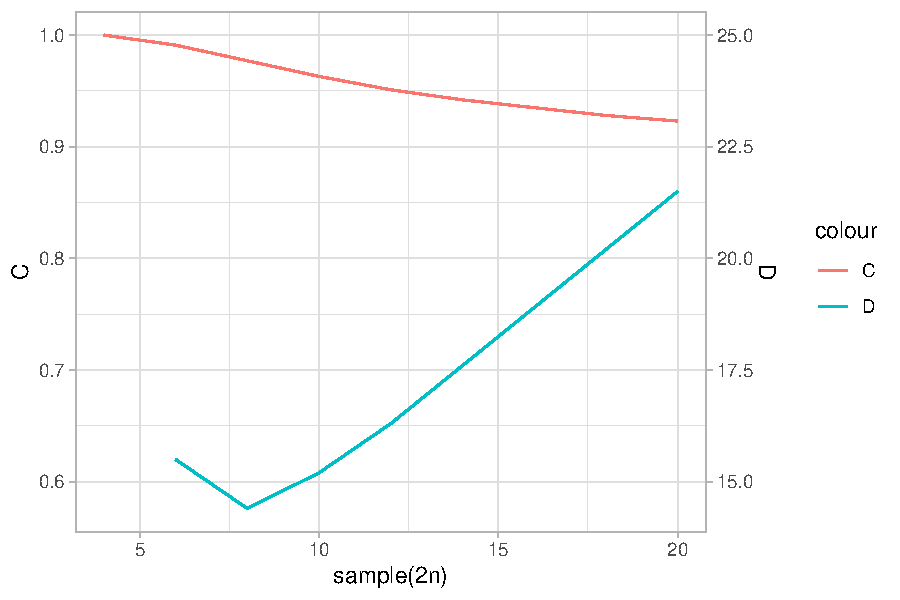
\includegraphics[height=2in,width=2.5in]{pic/Rplot01}
\begin{center} รูปที่1 ค่าความสอดคล้องและ ค่าความสามารถในการจำแนก เทียบจำนวนตัวอย่าง \end{center}

ในการทดลองที่ข้อมูลเป็นมีจำนวนคลาสสองคลาสและ เป็นข้อมูลที่สมดุลพบว่า AUC นั้นมีความสอดคล้องกับ ค่าความแม่นยำ และ AUC นั้นสามารถจำแนกเหตุการณ์ที่แตกต่างกันที่ค่าความแม่นยำไม่สามารถจำแนกได้มากกว่า และ เมื่อพิจารณามองความสามารถในการจำแนกนั้นพบว่ายิ่งจำนวนข้อมูลเยอะมากขึ้นนั้น ความสามารถในการจำแนกของ AUC จะสูงขึ้นด้วย แสดงดังรูปที่ 1
\subsection{ข้อมูลสองคลาสที่สมดุล}
\quad ข้อมูลไบนารีคลาสที่ไม่สมดุลโดยจะกำหนดให้มีตัวอย่างคลาสบวก 25\% และตัวอย่างคลาสลบ 75\% โดยข้อมูลที่ใช้จะมีจำนวน 4, 8, 12 และ 16 ตัวอย่างและยังคงใช้สูตรการคำนวณหาค่า AUC เหมือนเดิมและเนื่องจากจำนวนตัวอย่างนั้นไม่สมดุลทำให้การคำนวณค่าความแม่นยำจะเปลี่ยนจากเดิมที่ให้ 5 ตัวอย่างแรกเป็นคลาสลบและ 5 ตัวอย่างถัดไปเป็นคลาสบวกหรืออีกนัยหนึ่งคือแบ่งตรงกลางอย่างละครึ่ง แต่เมื่อข้อมูลนั้นมีขนาดไม่เท่ากันทำให้การแยกคลาสบวกและคลาสลบเป็น 75\% แรกเป็นคลาสลบ และ 25\% เป็นต่อมาเป็นคลาสบวกตามอัตราส่วนของข้อมูลเข้าที่เปลี่ยนไป

\begin{center} ตารางที่5 ความสอดคล้องกันของ AUC และ ความแม่นยำ(ไม่สมดุล) \end{center}
\begin{center}
\begin{tabular}{cccc}
  \hline
  2n&\specialcell{ค่า AUC และ\\ค่าความแม่นยำ\\สอดคล้องกัน}&\specialcell{ค่า AUC และ\\ค่าความแม่นยำ\\ไม่สอดคล้องกัน}&C \\
  \hline
  4&3&0&1 \\
  \hline  
  6&187&10&0.949 \\
  \hline  
  12&12,716&1,225&0.912 \\
  \hline  
  16&926,884&114,074&0.890 \\
  \hline  
\end{tabular}
\end{center}
\begin{center} ตารางที่6 ความสามารถในการจำแนกของค่า AUC และ ความแม่นยำ(ไม่สมดุล) \end{center}
\begin{center}
\begin{tabular}{cccc}
  \hline
  2n&\specialcell{ค่า AUC \\จำแนกได้ดีกว่า\\ค่าความแม่นยำ}&\specialcell{ค่าความแม่นยำ \\จำแนกได้ดีกว่า\\ค่า AUC}&D \\
  \hline
  4&3&0&$\infty$ \\
  \hline  
  8&159&10&15.9 \\
  \hline  
  12&8,986&489&18.4 \\
  \hline  
  16&559,751&25,969&21.6 \\
  \hline  
\end{tabular}
\end{center}

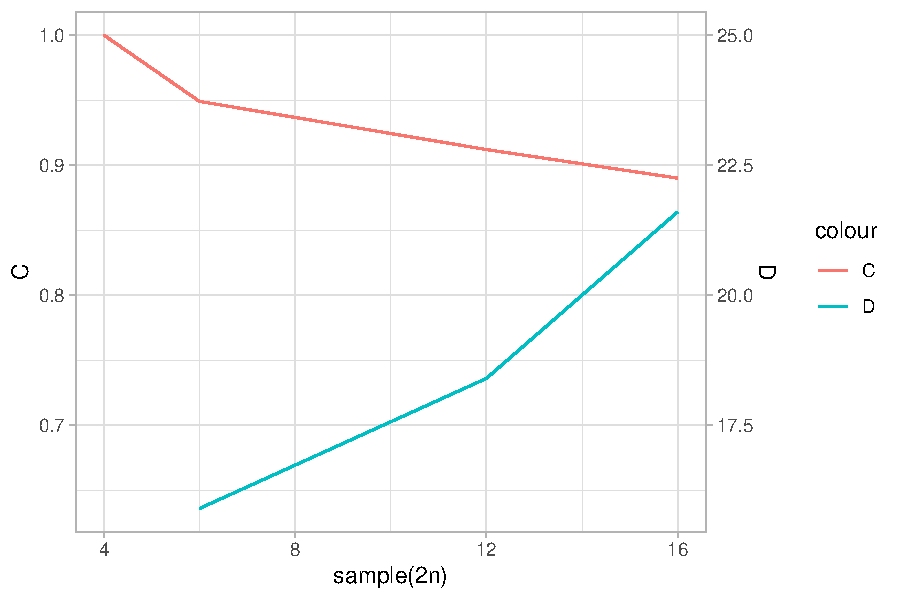
\includegraphics[height=2in,width=2.5in]{pic/Rplot02.pdf}
\begin{center} รูปที่2 ค่าความสอดคล้องและ ค่าความสามารถในการจำแนก เทียบจำนวนตัวอย่าง กรณีข้อมูลไม่สมดุล\end{center}
\begin{center} ตารางที่7 ความสอดคล้องและความสามารถในการจำแนกของค่า AUC และ ความแม่นยำ(ไม่สมดุล ขนาดข้อมูล 10 ตัวอย่าง) \end{center}
\begin{center}
\begin{tabular}{cccc}
\hline
คลาสบวก & คลาสลบ & C & D\\
\hline
1&9&1.0 &$\infty$\\\hline
2&8&0.926&22.3\\\hline
3&7&0.939&15.5\\\hline
4&6&0.956&14.9\\\hline
5&5&0.963&15.2\\\hline
\end{tabular}
\end{center}

และสุดท้ายเป็นการทดลองในหลายๆ อัตราส่วนของคลาสบวกและคลาสลบ โดยกำหนดให้มีข้อมูลทั้งหมด 10 ตัวอย่าง โดยเริ่มจากสมดุลคือมีทั้งหมดอย่างละ 5 ตัวอย่างจากนั้นเพิ่มและ ลดคลาสใดคลาสหนึ่งไปเรื่อยๆ จนไม่สามารถลดได้ ในกรณีนี้คือเหลือตัวเดียว

จากการทดลองทั้งสองไม่ว่าเป็นข้อมูลทั้งแบบที่สมดุลและ ไม่สมดุลก็ตามผลการทดลองยังคงเป็นไปในทิศทางเดียวกัน ทั้งในมุมความสอดคล้องที่ยังคงสอดคล้องกันสูง และในมุมความสามารถในการจำแนกที่ AUC มีความสามารถในการจำแนกสูงขึ้นเรื่อยๆ ตามขนาดของข้อมูลและ ยิ่งมีความสามารถในการจำแนกสูงมากขึ้นเมื่อข้อมูลเกิดความไม่สมดุลของทั้งสองคลาส


\section{การประยุกต์ใช้}
\quad จากการทดลองที่ผ่านมาได้เปรียบเทียบตัวประเมินประสิทธิภาพทั้งสองคือค่า AUC และ ค่าความแม่นยำ โดยว่า AUC มีประสิทธิภาพดีกว่าค่าความแม่นยำ แต่อย่างไรก็ตามในการใช้งานจริงทั้ง AUC และความแม่นยำไม่ใช่เป้าหมายสุดท้าย เช่น  ธนาคาร หรือ บริษัทประกันภัย อาจจะมีข้อมูลของลูกค้าอยู่มหาศาลโดยสิ่งที่ต้องการสุดท้ายคือการคาดการณ์การทำกำไรให้กับ บริษัท

สมมติว่าลูกค้าที่ถูกเก็บในฐานข้อมูลมีการเก็บด้วยแอตทริบิวต์จำนวนหนึ่งและลูกค้าแต่ละรายอาจเป็นผู้ซื้อหรือไม่ใช่ผู้ซื้อผลิตภัณฑ์บางอย่างเนื่องจากปัญหานี้เป็นปัญหาการจำแนกแบบไบนารี่ ลูกค้าจะได้รับการติดต่อจากแคมเปญการส่งเสริมการขายสำหรับลูกค้าแต่ละรายโดย บริษัทต้องคาดการณ์ว่าในสินค้าชนิดๆ หนึ่งนั้นลูกค้าแต่ละรายมีความต้องการสินค้านั้นมากเพียงใด และ ต้องเพิ่มโอกาสการซื้อมากน้อยเพียงใด

อย่างไรก็ตามการประยุกต์ใช้ บริษัท อาจต้องการโปรโมตเพียงเล็กน้อยให้กับลูกค้าที่มีแนวโน้มสูงที่สุดที่คาดการณ์ไว้ และต้องโปรโมตมากขึ้นสำหรับลูกค้าที่มีแนวโน้มลดลง ซึ่งทำให้กำไรที่ได้ต่อลูกค้าแต่ละคนนั้นต่างกันไปด้วยซึ่งในความเป็นจริง ก่อให้เกิดผลดีต่อรายได้ของบริษัทเพราะสามารถลดการโปรโมตเกินจำเป็นสำหรับลูกค้าที่มีแนวโน้มจะซื้อสินค้าสูงๆ อยู่แล้ว เช่น ลูกค้าที่มีแนวโน้มจะซื้อสินค้าสูงสุด 10\% แรกนั้นอาจจะเป็นลูกค้าที่มีการซื้อสินค้าเป็นประจำในการโปรโมตสินค้าที่ลูกค้ากลุ่มนี้ซื้อเป็นประจำอยู่แล้วอาจไม่จำเป็น และเพิ่มโอกาสให้ลูกค้าที่มีแนวโน้มลดลงมามีโอกาสซื้อสินค้ามากขึ้นด้วย 
\section{สรุป}
\quad ในบทความนี้ได้ให้คำจำกัดความอย่างเป็นทางการเกี่ยวกับความสอดคล้องและ ความสามารถในการจำแนก เพื่อใช้ประเมินผลสำหรับขั้นตอนวิธีการเรียนรู้ในปัญหาการจำแนก กำหนดรูปแบบและเกณฑ์ที่ใช้สำหรับการเปรียบเทียบตัวประเมินประสิทธิภาพทั้งสอง และแสดงให้เห็นอย่างชัดเจนว่า AUC นั้นเป็นตัวประเมินประสิทธิภาพที่ดีกว่าค่าความแม่นยำ และได้นำไปเปรียบเทียบกับเหตุการณ์จริงในธุรกิจเพื่อแสดงผลลัพธ์ที่น่าสนใจว่า AUC เกี่ยวข้องโดยตรงกับกำไรสุทธิมากกว่าค่าความแม่นยำในการตลาดทางตรง

การเพิ่มประสิทธิภาพ AUC นั้นเป็นที่ต้องการมากกว่าการเพิ่มความแม่นยำในการนำขั้นตอนวิธีการเรียนรู้สำหรับปัญหาการจำแนกรวมถึงการทำเหมืองข้อมูลที่จะนำไปประยุกต์ใช้ในโลกความเป็นจริง
\renewcommand\refname{ข้อมูลอ้างอิง}

\begin{thebibliography}{9}

\bibitem{latexcompanion} 
Cortes, Corinna and Mohri, Mehryar. \textit{{AUC} {Optimization} vs. {Error} {Rate} {Minimization}}. Florham Park, NJ 07932, USA

\bibitem{latexcompanion} 
Ling, Charles X and Huang, Jin and Zhang, Harry. \textit{{AUC}: a {Statistically} {Consistent} and more {Discriminating} {Measure} than {Accuracy}}. Fredericton, NB, Canada

\bibitem{latexcompanion} 
{Jin Huang} and Ling, C.X. \textit{Using {AUC} and accuracy in evaluating learning algorithms}. London, Ontario, Canada


\end{thebibliography}

\end{document}


















































